% RoboForge v1.1 addendum (DECISIONS D-131, D-133). Build: make addendum (Tectonic, the
% v1.0.0 toolchain). Every number in the prose is a generated macro \ax{key}
% (generated/numbers.tex) and every table and figure is generated (generated/), from the three
% hash-pinned extension results only. The v1.0.0 report (paper/main.pdf) is unchanged.
\documentclass[10pt,a4paper]{article}
\usepackage{fontspec}
\usepackage[margin=2.2cm]{geometry}
\usepackage{amsmath,amssymb}
\usepackage{booktabs,array,graphicx,xcolor}
\usepackage[numbers,sort&compress]{natbib}
\usepackage[hidelinks]{hyperref}
\usepackage[font=small,labelfont=bf]{caption}
\usepackage{placeins}

% Generated results: \ax{key} expands a pinned value; an undefined key is an error.
% Generated by scripts/addendum_assets.py (DECISIONS D-133). Do not edit.
% Sources (path sha256):
%   reports/session13/x1_clamp/results.json ad50368645b96fb87489310243535f97694b1e47a2ff993915b039b2199a5ee7
%   reports/session14/x3/results.json 4299a14930790bfdb2f91d7a3216c9bd7f6db1fa2171469a29bfed3c5c5b71d1
%   reports/session17/x2/results.json 30c01f551333feafba70bfa4c9c6a414eda691f179800022d3871776be2df238
\expandafter\def\csname ax@x1.prim.d\endcsname{\ensuremath{-}40.0}
\expandafter\def\csname ax@x1.prim.lo\endcsname{\ensuremath{-}54.0}
\expandafter\def\csname ax@x1.prim.hi\endcsname{\ensuremath{-}25.3}
\expandafter\def\csname ax@x1.prim.sep\endcsname{separated (\ensuremath{-})}
\expandafter\def\csname ax@x1.prim.f.d\endcsname{\ensuremath{-}40.0}
\expandafter\def\csname ax@x1.prim.f.lo\endcsname{\ensuremath{-}54.0}
\expandafter\def\csname ax@x1.prim.f.hi\endcsname{\ensuremath{-}26.0}
\expandafter\def\csname ax@x1.prim.f.sep\endcsname{separated (\ensuremath{-})}
\expandafter\def\csname ax@x1.sup.d\endcsname{\ensuremath{+}0.0}
\expandafter\def\csname ax@x1.sup.lo\endcsname{\ensuremath{-}4.0}
\expandafter\def\csname ax@x1.sup.hi\endcsname{\ensuremath{+}4.0}
\expandafter\def\csname ax@x1.sup.sep\endcsname{not separated}
\expandafter\def\csname ax@x1.base.lift.d\endcsname{\ensuremath{+}0.0}
\expandafter\def\csname ax@x1.base.lift.lo\endcsname{\ensuremath{+}0.0}
\expandafter\def\csname ax@x1.base.lift.hi\endcsname{\ensuremath{+}0.0}
\expandafter\def\csname ax@x1.base.lift.sep\endcsname{not separated}
\expandafter\def\csname ax@x1.base.can.d\endcsname{\ensuremath{+}0.0}
\expandafter\def\csname ax@x1.base.can.lo\endcsname{\ensuremath{+}0.0}
\expandafter\def\csname ax@x1.base.can.hi\endcsname{\ensuremath{+}0.0}
\expandafter\def\csname ax@x1.base.can.sep\endcsname{not separated}
\expandafter\def\csname ax@x1.nevals\endcsname{45}
\expandafter\def\csname ax@x1.B\endcsname{10,000}
\expandafter\def\csname ax@x1.lift.nstates\endcsname{50}
\expandafter\def\csname ax@x1.lift.diff.base.succ\endcsname{99.3}
\expandafter\def\csname ax@x1.lift.diff.base.lo\endcsname{96.0}
\expandafter\def\csname ax@x1.lift.diff.base.hi\endcsname{100.0}
\expandafter\def\csname ax@x1.lift.diff.base.perseed\endcsname{100, 98, 100}
\expandafter\def\csname ax@x1.lift.diff.base.nseeds\endcsname{3}
\expandafter\def\csname ax@x1.lift.diff.base.nstates\endcsname{50}
\expandafter\def\csname ax@x1.lift.diff.cube.succ\endcsname{85.3}
\expandafter\def\csname ax@x1.lift.diff.cube.lo\endcsname{76.0}
\expandafter\def\csname ax@x1.lift.diff.cube.hi\endcsname{93.3}
\expandafter\def\csname ax@x1.lift.diff.cube.perseed\endcsname{86, 84, 86}
\expandafter\def\csname ax@x1.lift.diff.cube.nseeds\endcsname{3}
\expandafter\def\csname ax@x1.lift.diff.cube.nstates\endcsname{50}
\expandafter\def\csname ax@x1.lift.diff.arm.succ\endcsname{88.0}
\expandafter\def\csname ax@x1.lift.diff.arm.lo\endcsname{79.3}
\expandafter\def\csname ax@x1.lift.diff.arm.hi\endcsname{95.3}
\expandafter\def\csname ax@x1.lift.diff.arm.perseed\endcsname{86, 92, 86}
\expandafter\def\csname ax@x1.lift.diff.arm.nseeds\endcsname{3}
\expandafter\def\csname ax@x1.lift.diff.arm.nstates\endcsname{50}
\expandafter\def\csname ax@x1.lift.chunk.base.succ\endcsname{100.0}
\expandafter\def\csname ax@x1.lift.chunk.base.lo\endcsname{100.0}
\expandafter\def\csname ax@x1.lift.chunk.base.hi\endcsname{100.0}
\expandafter\def\csname ax@x1.lift.chunk.base.perseed\endcsname{100, 100, 100}
\expandafter\def\csname ax@x1.lift.chunk.base.nseeds\endcsname{3}
\expandafter\def\csname ax@x1.lift.chunk.base.nstates\endcsname{50}
\expandafter\def\csname ax@x1.lift.chunk.cube.succ\endcsname{54.7}
\expandafter\def\csname ax@x1.lift.chunk.cube.lo\endcsname{33.3}
\expandafter\def\csname ax@x1.lift.chunk.cube.hi\endcsname{75.3}
\expandafter\def\csname ax@x1.lift.chunk.cube.perseed\endcsname{34, 74, 56}
\expandafter\def\csname ax@x1.lift.chunk.cube.nseeds\endcsname{3}
\expandafter\def\csname ax@x1.lift.chunk.cube.nstates\endcsname{50}
\expandafter\def\csname ax@x1.lift.chunk.arm.succ\endcsname{48.7}
\expandafter\def\csname ax@x1.lift.chunk.arm.lo\endcsname{36.0}
\expandafter\def\csname ax@x1.lift.chunk.arm.hi\endcsname{61.3}
\expandafter\def\csname ax@x1.lift.chunk.arm.perseed\endcsname{52, 52, 42}
\expandafter\def\csname ax@x1.lift.chunk.arm.nseeds\endcsname{3}
\expandafter\def\csname ax@x1.lift.chunk.arm.nstates\endcsname{50}
\expandafter\def\csname ax@x1.lift.chunkc.base.succ\endcsname{100.0}
\expandafter\def\csname ax@x1.lift.chunkc.base.lo\endcsname{100.0}
\expandafter\def\csname ax@x1.lift.chunkc.base.hi\endcsname{100.0}
\expandafter\def\csname ax@x1.lift.chunkc.base.perseed\endcsname{100, 100, 100}
\expandafter\def\csname ax@x1.lift.chunkc.base.nseeds\endcsname{3}
\expandafter\def\csname ax@x1.lift.chunkc.base.nstates\endcsname{50}
\expandafter\def\csname ax@x1.lift.chunkc.cube.succ\endcsname{54.7}
\expandafter\def\csname ax@x1.lift.chunkc.cube.lo\endcsname{33.3}
\expandafter\def\csname ax@x1.lift.chunkc.cube.hi\endcsname{75.3}
\expandafter\def\csname ax@x1.lift.chunkc.cube.perseed\endcsname{34, 74, 56}
\expandafter\def\csname ax@x1.lift.chunkc.cube.nseeds\endcsname{3}
\expandafter\def\csname ax@x1.lift.chunkc.cube.nstates\endcsname{50}
\expandafter\def\csname ax@x1.lift.chunkc.arm.succ\endcsname{48.7}
\expandafter\def\csname ax@x1.lift.chunkc.arm.lo\endcsname{36.0}
\expandafter\def\csname ax@x1.lift.chunkc.arm.hi\endcsname{62.0}
\expandafter\def\csname ax@x1.lift.chunkc.arm.perseed\endcsname{52, 52, 42}
\expandafter\def\csname ax@x1.lift.chunkc.arm.nseeds\endcsname{3}
\expandafter\def\csname ax@x1.lift.chunkc.arm.nstates\endcsname{50}
\expandafter\def\csname ax@x1.lift.bcmlp.base.succ\endcsname{98.0}
\expandafter\def\csname ax@x1.lift.bcmlp.base.lo\endcsname{92.0}
\expandafter\def\csname ax@x1.lift.bcmlp.base.hi\endcsname{100.0}
\expandafter\def\csname ax@x1.lift.bcmlp.base.perseed\endcsname{94, 100, 100}
\expandafter\def\csname ax@x1.lift.bcmlp.base.nseeds\endcsname{3}
\expandafter\def\csname ax@x1.lift.bcmlp.base.nstates\endcsname{50}
\expandafter\def\csname ax@x1.lift.bcmlp.cube.succ\endcsname{52.7}
\expandafter\def\csname ax@x1.lift.bcmlp.cube.lo\endcsname{35.3}
\expandafter\def\csname ax@x1.lift.bcmlp.cube.hi\endcsname{69.3}
\expandafter\def\csname ax@x1.lift.bcmlp.cube.perseed\endcsname{36, 60, 62}
\expandafter\def\csname ax@x1.lift.bcmlp.cube.nseeds\endcsname{3}
\expandafter\def\csname ax@x1.lift.bcmlp.cube.nstates\endcsname{50}
\expandafter\def\csname ax@x1.lift.bcmlp.arm.succ\endcsname{22.7}
\expandafter\def\csname ax@x1.lift.bcmlp.arm.lo\endcsname{12.0}
\expandafter\def\csname ax@x1.lift.bcmlp.arm.hi\endcsname{34.0}
\expandafter\def\csname ax@x1.lift.bcmlp.arm.perseed\endcsname{18, 24, 26}
\expandafter\def\csname ax@x1.lift.bcmlp.arm.nseeds\endcsname{3}
\expandafter\def\csname ax@x1.lift.bcmlp.arm.nstates\endcsname{50}
\expandafter\def\csname ax@x1.lift.bcmlpc.base.succ\endcsname{98.0}
\expandafter\def\csname ax@x1.lift.bcmlpc.base.lo\endcsname{92.0}
\expandafter\def\csname ax@x1.lift.bcmlpc.base.hi\endcsname{100.0}
\expandafter\def\csname ax@x1.lift.bcmlpc.base.perseed\endcsname{94, 100, 100}
\expandafter\def\csname ax@x1.lift.bcmlpc.base.nseeds\endcsname{3}
\expandafter\def\csname ax@x1.lift.bcmlpc.base.nstates\endcsname{50}
\expandafter\def\csname ax@x1.lift.bcmlpc.cube.succ\endcsname{52.0}
\expandafter\def\csname ax@x1.lift.bcmlpc.cube.lo\endcsname{34.0}
\expandafter\def\csname ax@x1.lift.bcmlpc.cube.hi\endcsname{69.3}
\expandafter\def\csname ax@x1.lift.bcmlpc.cube.perseed\endcsname{34, 60, 62}
\expandafter\def\csname ax@x1.lift.bcmlpc.cube.nseeds\endcsname{3}
\expandafter\def\csname ax@x1.lift.bcmlpc.cube.nstates\endcsname{50}
\expandafter\def\csname ax@x1.lift.bcmlpc.arm.succ\endcsname{22.7}
\expandafter\def\csname ax@x1.lift.bcmlpc.arm.lo\endcsname{13.3}
\expandafter\def\csname ax@x1.lift.bcmlpc.arm.hi\endcsname{33.3}
\expandafter\def\csname ax@x1.lift.bcmlpc.arm.perseed\endcsname{20, 24, 24}
\expandafter\def\csname ax@x1.lift.bcmlpc.arm.nseeds\endcsname{3}
\expandafter\def\csname ax@x1.lift.bcmlpc.arm.nstates\endcsname{50}
\expandafter\def\csname ax@x1.lift.bcrnn.base.succ\endcsname{100.0}
\expandafter\def\csname ax@x1.lift.bcrnn.base.lo\endcsname{100.0}
\expandafter\def\csname ax@x1.lift.bcrnn.base.hi\endcsname{100.0}
\expandafter\def\csname ax@x1.lift.bcrnn.base.perseed\endcsname{100, 100, 100}
\expandafter\def\csname ax@x1.lift.bcrnn.base.nseeds\endcsname{3}
\expandafter\def\csname ax@x1.lift.bcrnn.base.nstates\endcsname{50}
\expandafter\def\csname ax@x1.lift.bcrnn.cube.succ\endcsname{96.0}
\expandafter\def\csname ax@x1.lift.bcrnn.cube.lo\endcsname{88.0}
\expandafter\def\csname ax@x1.lift.bcrnn.cube.hi\endcsname{100.0}
\expandafter\def\csname ax@x1.lift.bcrnn.cube.perseed\endcsname{90, 98, 100}
\expandafter\def\csname ax@x1.lift.bcrnn.cube.nseeds\endcsname{3}
\expandafter\def\csname ax@x1.lift.bcrnn.cube.nstates\endcsname{50}
\expandafter\def\csname ax@x1.lift.bcrnn.arm.succ\endcsname{50.0}
\expandafter\def\csname ax@x1.lift.bcrnn.arm.lo\endcsname{36.0}
\expandafter\def\csname ax@x1.lift.bcrnn.arm.hi\endcsname{64.0}
\expandafter\def\csname ax@x1.lift.bcrnn.arm.perseed\endcsname{46, 46, 58}
\expandafter\def\csname ax@x1.lift.bcrnn.arm.nseeds\endcsname{3}
\expandafter\def\csname ax@x1.lift.bcrnn.arm.nstates\endcsname{50}
\expandafter\def\csname ax@x1.lift.bcrnnc.base.succ\endcsname{100.0}
\expandafter\def\csname ax@x1.lift.bcrnnc.base.lo\endcsname{100.0}
\expandafter\def\csname ax@x1.lift.bcrnnc.base.hi\endcsname{100.0}
\expandafter\def\csname ax@x1.lift.bcrnnc.base.perseed\endcsname{100, 100, 100}
\expandafter\def\csname ax@x1.lift.bcrnnc.base.nseeds\endcsname{3}
\expandafter\def\csname ax@x1.lift.bcrnnc.base.nstates\endcsname{50}
\expandafter\def\csname ax@x1.lift.bcrnnc.cube.succ\endcsname{96.0}
\expandafter\def\csname ax@x1.lift.bcrnnc.cube.lo\endcsname{88.0}
\expandafter\def\csname ax@x1.lift.bcrnnc.cube.hi\endcsname{100.0}
\expandafter\def\csname ax@x1.lift.bcrnnc.cube.perseed\endcsname{90, 98, 100}
\expandafter\def\csname ax@x1.lift.bcrnnc.cube.nseeds\endcsname{3}
\expandafter\def\csname ax@x1.lift.bcrnnc.cube.nstates\endcsname{50}
\expandafter\def\csname ax@x1.lift.bcrnnc.arm.succ\endcsname{49.3}
\expandafter\def\csname ax@x1.lift.bcrnnc.arm.lo\endcsname{35.3}
\expandafter\def\csname ax@x1.lift.bcrnnc.arm.hi\endcsname{64.0}
\expandafter\def\csname ax@x1.lift.bcrnnc.arm.perseed\endcsname{46, 44, 58}
\expandafter\def\csname ax@x1.lift.bcrnnc.arm.nseeds\endcsname{3}
\expandafter\def\csname ax@x1.lift.bcrnnc.arm.nstates\endcsname{50}
\expandafter\def\csname ax@x1.lift.dd.bcmlpc.cube.d\endcsname{\ensuremath{-}32.0}
\expandafter\def\csname ax@x1.lift.dd.bcmlpc.cube.lo\endcsname{\ensuremath{-}49.3}
\expandafter\def\csname ax@x1.lift.dd.bcmlpc.cube.hi\endcsname{\ensuremath{-}15.3}
\expandafter\def\csname ax@x1.lift.dd.bcmlpc.cube.sep\endcsname{separated (\ensuremath{-})}
\expandafter\def\csname ax@x1.lift.dd.bcmlp.cube.f.d\endcsname{\ensuremath{-}31.3}
\expandafter\def\csname ax@x1.lift.dd.bcmlp.cube.f.lo\endcsname{\ensuremath{-}48.0}
\expandafter\def\csname ax@x1.lift.dd.bcmlp.cube.f.hi\endcsname{\ensuremath{-}15.3}
\expandafter\def\csname ax@x1.lift.dd.bcmlp.cube.f.sep\endcsname{separated (\ensuremath{-})}
\expandafter\def\csname ax@x1.lift.dd.bcmlpc.arm.d\endcsname{\ensuremath{-}64.0}
\expandafter\def\csname ax@x1.lift.dd.bcmlpc.arm.lo\endcsname{\ensuremath{-}76.7}
\expandafter\def\csname ax@x1.lift.dd.bcmlpc.arm.hi\endcsname{\ensuremath{-}51.3}
\expandafter\def\csname ax@x1.lift.dd.bcmlpc.arm.sep\endcsname{separated (\ensuremath{-})}
\expandafter\def\csname ax@x1.lift.dd.bcmlp.arm.f.d\endcsname{\ensuremath{-}64.0}
\expandafter\def\csname ax@x1.lift.dd.bcmlp.arm.f.lo\endcsname{\ensuremath{-}76.7}
\expandafter\def\csname ax@x1.lift.dd.bcmlp.arm.f.hi\endcsname{\ensuremath{-}50.7}
\expandafter\def\csname ax@x1.lift.dd.bcmlp.arm.f.sep\endcsname{separated (\ensuremath{-})}
\expandafter\def\csname ax@x1.lift.dd.bcrnnc.cube.d\endcsname{\ensuremath{+}10.0}
\expandafter\def\csname ax@x1.lift.dd.bcrnnc.cube.lo\endcsname{\ensuremath{-}0.7}
\expandafter\def\csname ax@x1.lift.dd.bcrnnc.cube.hi\endcsname{\ensuremath{+}20.7}
\expandafter\def\csname ax@x1.lift.dd.bcrnnc.cube.sep\endcsname{not separated}
\expandafter\def\csname ax@x1.lift.dd.bcrnn.cube.f.d\endcsname{\ensuremath{+}10.0}
\expandafter\def\csname ax@x1.lift.dd.bcrnn.cube.f.lo\endcsname{\ensuremath{-}0.7}
\expandafter\def\csname ax@x1.lift.dd.bcrnn.cube.f.hi\endcsname{\ensuremath{+}20.7}
\expandafter\def\csname ax@x1.lift.dd.bcrnn.cube.f.sep\endcsname{not separated}
\expandafter\def\csname ax@x1.lift.dd.bcrnnc.arm.d\endcsname{\ensuremath{-}39.3}
\expandafter\def\csname ax@x1.lift.dd.bcrnnc.arm.lo\endcsname{\ensuremath{-}54.7}
\expandafter\def\csname ax@x1.lift.dd.bcrnnc.arm.hi\endcsname{\ensuremath{-}24.7}
\expandafter\def\csname ax@x1.lift.dd.bcrnnc.arm.sep\endcsname{separated (\ensuremath{-})}
\expandafter\def\csname ax@x1.lift.dd.bcrnn.arm.f.d\endcsname{\ensuremath{-}38.7}
\expandafter\def\csname ax@x1.lift.dd.bcrnn.arm.f.lo\endcsname{\ensuremath{-}53.3}
\expandafter\def\csname ax@x1.lift.dd.bcrnn.arm.f.hi\endcsname{\ensuremath{-}24.0}
\expandafter\def\csname ax@x1.lift.dd.bcrnn.arm.f.sep\endcsname{separated (\ensuremath{-})}
\expandafter\def\csname ax@x1.lift.dd.chunkc.cube.d\endcsname{\ensuremath{-}31.3}
\expandafter\def\csname ax@x1.lift.dd.chunkc.cube.lo\endcsname{\ensuremath{-}54.0}
\expandafter\def\csname ax@x1.lift.dd.chunkc.cube.hi\endcsname{\ensuremath{-}10.0}
\expandafter\def\csname ax@x1.lift.dd.chunkc.cube.sep\endcsname{separated (\ensuremath{-})}
\expandafter\def\csname ax@x1.lift.dd.chunk.cube.f.d\endcsname{\ensuremath{-}31.3}
\expandafter\def\csname ax@x1.lift.dd.chunk.cube.f.lo\endcsname{\ensuremath{-}54.0}
\expandafter\def\csname ax@x1.lift.dd.chunk.cube.f.hi\endcsname{\ensuremath{-}10.0}
\expandafter\def\csname ax@x1.lift.dd.chunk.cube.f.sep\endcsname{separated (\ensuremath{-})}
\expandafter\def\csname ax@x1.lift.dd.chunkc.arm.d\endcsname{\ensuremath{-}40.0}
\expandafter\def\csname ax@x1.lift.dd.chunkc.arm.lo\endcsname{\ensuremath{-}54.0}
\expandafter\def\csname ax@x1.lift.dd.chunkc.arm.hi\endcsname{\ensuremath{-}25.3}
\expandafter\def\csname ax@x1.lift.dd.chunkc.arm.sep\endcsname{separated (\ensuremath{-})}
\expandafter\def\csname ax@x1.lift.dd.chunk.arm.f.d\endcsname{\ensuremath{-}40.0}
\expandafter\def\csname ax@x1.lift.dd.chunk.arm.f.lo\endcsname{\ensuremath{-}54.0}
\expandafter\def\csname ax@x1.lift.dd.chunk.arm.f.hi\endcsname{\ensuremath{-}26.0}
\expandafter\def\csname ax@x1.lift.dd.chunk.arm.f.sep\endcsname{separated (\ensuremath{-})}
\expandafter\def\csname ax@x1.lift.chg.bcmlpc.base\endcsname{12.4}
\expandafter\def\csname ax@x1.lift.chg.bcmlpc.cube\endcsname{63.8}
\expandafter\def\csname ax@x1.lift.chg.bcmlpc.arm\endcsname{72.5}
\expandafter\def\csname ax@x1.lift.chg.bcrnnc.base\endcsname{0.0}
\expandafter\def\csname ax@x1.lift.chg.bcrnnc.cube\endcsname{0.2}
\expandafter\def\csname ax@x1.lift.chg.bcrnnc.arm\endcsname{3.2}
\expandafter\def\csname ax@x1.lift.chg.chunkc.base\endcsname{0.0}
\expandafter\def\csname ax@x1.lift.chg.chunkc.cube\endcsname{54.2}
\expandafter\def\csname ax@x1.lift.chg.chunkc.arm\endcsname{51.7}
\expandafter\def\csname ax@x1.can.nstates\endcsname{50}
\expandafter\def\csname ax@x1.can.diff.base.succ\endcsname{92.0}
\expandafter\def\csname ax@x1.can.diff.base.lo\endcsname{85.3}
\expandafter\def\csname ax@x1.can.diff.base.hi\endcsname{98.0}
\expandafter\def\csname ax@x1.can.diff.base.perseed\endcsname{90, 94, 92}
\expandafter\def\csname ax@x1.can.diff.base.nseeds\endcsname{3}
\expandafter\def\csname ax@x1.can.diff.base.nstates\endcsname{50}
\expandafter\def\csname ax@x1.can.diff.arm.succ\endcsname{71.3}
\expandafter\def\csname ax@x1.can.diff.arm.lo\endcsname{58.0}
\expandafter\def\csname ax@x1.can.diff.arm.hi\endcsname{84.0}
\expandafter\def\csname ax@x1.can.diff.arm.perseed\endcsname{66, 68, 80}
\expandafter\def\csname ax@x1.can.diff.arm.nseeds\endcsname{3}
\expandafter\def\csname ax@x1.can.diff.arm.nstates\endcsname{50}
\expandafter\def\csname ax@x1.can.chunk.base.succ\endcsname{95.3}
\expandafter\def\csname ax@x1.can.chunk.base.lo\endcsname{89.3}
\expandafter\def\csname ax@x1.can.chunk.base.hi\endcsname{100.0}
\expandafter\def\csname ax@x1.can.chunk.base.perseed\endcsname{94, 94, 98}
\expandafter\def\csname ax@x1.can.chunk.base.nseeds\endcsname{3}
\expandafter\def\csname ax@x1.can.chunk.base.nstates\endcsname{50}
\expandafter\def\csname ax@x1.can.chunk.arm.succ\endcsname{79.3}
\expandafter\def\csname ax@x1.can.chunk.arm.lo\endcsname{66.0}
\expandafter\def\csname ax@x1.can.chunk.arm.hi\endcsname{90.7}
\expandafter\def\csname ax@x1.can.chunk.arm.perseed\endcsname{82, 68, 88}
\expandafter\def\csname ax@x1.can.chunk.arm.nseeds\endcsname{3}
\expandafter\def\csname ax@x1.can.chunk.arm.nstates\endcsname{50}
\expandafter\def\csname ax@x1.can.chunkc.base.succ\endcsname{95.3}
\expandafter\def\csname ax@x1.can.chunkc.base.lo\endcsname{89.3}
\expandafter\def\csname ax@x1.can.chunkc.base.hi\endcsname{100.0}
\expandafter\def\csname ax@x1.can.chunkc.base.perseed\endcsname{94, 94, 98}
\expandafter\def\csname ax@x1.can.chunkc.base.nseeds\endcsname{3}
\expandafter\def\csname ax@x1.can.chunkc.base.nstates\endcsname{50}
\expandafter\def\csname ax@x1.can.chunkc.arm.succ\endcsname{79.3}
\expandafter\def\csname ax@x1.can.chunkc.arm.lo\endcsname{66.0}
\expandafter\def\csname ax@x1.can.chunkc.arm.hi\endcsname{90.7}
\expandafter\def\csname ax@x1.can.chunkc.arm.perseed\endcsname{82, 68, 88}
\expandafter\def\csname ax@x1.can.chunkc.arm.nseeds\endcsname{3}
\expandafter\def\csname ax@x1.can.chunkc.arm.nstates\endcsname{50}
\expandafter\def\csname ax@x1.can.bcmlp.base.succ\endcsname{69.3}
\expandafter\def\csname ax@x1.can.bcmlp.base.lo\endcsname{56.0}
\expandafter\def\csname ax@x1.can.bcmlp.base.hi\endcsname{82.0}
\expandafter\def\csname ax@x1.can.bcmlp.base.perseed\endcsname{68, 78, 62}
\expandafter\def\csname ax@x1.can.bcmlp.base.nseeds\endcsname{3}
\expandafter\def\csname ax@x1.can.bcmlp.base.nstates\endcsname{50}
\expandafter\def\csname ax@x1.can.bcmlp.arm.succ\endcsname{30.0}
\expandafter\def\csname ax@x1.can.bcmlp.arm.lo\endcsname{19.3}
\expandafter\def\csname ax@x1.can.bcmlp.arm.hi\endcsname{41.3}
\expandafter\def\csname ax@x1.can.bcmlp.arm.perseed\endcsname{26, 36, 28}
\expandafter\def\csname ax@x1.can.bcmlp.arm.nseeds\endcsname{3}
\expandafter\def\csname ax@x1.can.bcmlp.arm.nstates\endcsname{50}
\expandafter\def\csname ax@x1.can.bcmlpc.base.succ\endcsname{69.3}
\expandafter\def\csname ax@x1.can.bcmlpc.base.lo\endcsname{56.0}
\expandafter\def\csname ax@x1.can.bcmlpc.base.hi\endcsname{82.0}
\expandafter\def\csname ax@x1.can.bcmlpc.base.perseed\endcsname{68, 78, 62}
\expandafter\def\csname ax@x1.can.bcmlpc.base.nseeds\endcsname{3}
\expandafter\def\csname ax@x1.can.bcmlpc.base.nstates\endcsname{50}
\expandafter\def\csname ax@x1.can.bcmlpc.arm.succ\endcsname{30.0}
\expandafter\def\csname ax@x1.can.bcmlpc.arm.lo\endcsname{19.3}
\expandafter\def\csname ax@x1.can.bcmlpc.arm.hi\endcsname{41.3}
\expandafter\def\csname ax@x1.can.bcmlpc.arm.perseed\endcsname{26, 36, 28}
\expandafter\def\csname ax@x1.can.bcmlpc.arm.nseeds\endcsname{3}
\expandafter\def\csname ax@x1.can.bcmlpc.arm.nstates\endcsname{50}
\expandafter\def\csname ax@x1.can.bcrnn.base.succ\endcsname{96.7}
\expandafter\def\csname ax@x1.can.bcrnn.base.lo\endcsname{91.3}
\expandafter\def\csname ax@x1.can.bcrnn.base.hi\endcsname{100.0}
\expandafter\def\csname ax@x1.can.bcrnn.base.perseed\endcsname{94, 98, 98}
\expandafter\def\csname ax@x1.can.bcrnn.base.nseeds\endcsname{3}
\expandafter\def\csname ax@x1.can.bcrnn.base.nstates\endcsname{50}
\expandafter\def\csname ax@x1.can.bcrnn.arm.succ\endcsname{53.3}
\expandafter\def\csname ax@x1.can.bcrnn.arm.lo\endcsname{41.3}
\expandafter\def\csname ax@x1.can.bcrnn.arm.hi\endcsname{66.0}
\expandafter\def\csname ax@x1.can.bcrnn.arm.perseed\endcsname{54, 56, 50}
\expandafter\def\csname ax@x1.can.bcrnn.arm.nseeds\endcsname{3}
\expandafter\def\csname ax@x1.can.bcrnn.arm.nstates\endcsname{50}
\expandafter\def\csname ax@x1.can.bcrnnc.base.succ\endcsname{96.7}
\expandafter\def\csname ax@x1.can.bcrnnc.base.lo\endcsname{91.3}
\expandafter\def\csname ax@x1.can.bcrnnc.base.hi\endcsname{100.0}
\expandafter\def\csname ax@x1.can.bcrnnc.base.perseed\endcsname{94, 98, 98}
\expandafter\def\csname ax@x1.can.bcrnnc.base.nseeds\endcsname{3}
\expandafter\def\csname ax@x1.can.bcrnnc.base.nstates\endcsname{50}
\expandafter\def\csname ax@x1.can.bcrnnc.arm.succ\endcsname{53.3}
\expandafter\def\csname ax@x1.can.bcrnnc.arm.lo\endcsname{41.3}
\expandafter\def\csname ax@x1.can.bcrnnc.arm.hi\endcsname{66.0}
\expandafter\def\csname ax@x1.can.bcrnnc.arm.perseed\endcsname{54, 56, 50}
\expandafter\def\csname ax@x1.can.bcrnnc.arm.nseeds\endcsname{3}
\expandafter\def\csname ax@x1.can.bcrnnc.arm.nstates\endcsname{50}
\expandafter\def\csname ax@x1.can.dd.bcmlpc.arm.d\endcsname{\ensuremath{-}18.7}
\expandafter\def\csname ax@x1.can.dd.bcmlpc.arm.lo\endcsname{\ensuremath{-}36.0}
\expandafter\def\csname ax@x1.can.dd.bcmlpc.arm.hi\endcsname{\ensuremath{-}0.7}
\expandafter\def\csname ax@x1.can.dd.bcmlpc.arm.sep\endcsname{separated (\ensuremath{-})}
\expandafter\def\csname ax@x1.can.dd.bcmlp.arm.f.d\endcsname{\ensuremath{-}18.7}
\expandafter\def\csname ax@x1.can.dd.bcmlp.arm.f.lo\endcsname{\ensuremath{-}36.0}
\expandafter\def\csname ax@x1.can.dd.bcmlp.arm.f.hi\endcsname{\ensuremath{-}0.7}
\expandafter\def\csname ax@x1.can.dd.bcmlp.arm.f.sep\endcsname{separated (\ensuremath{-})}
\expandafter\def\csname ax@x1.can.dd.bcrnnc.arm.d\endcsname{\ensuremath{-}22.7}
\expandafter\def\csname ax@x1.can.dd.bcrnnc.arm.lo\endcsname{\ensuremath{-}39.3}
\expandafter\def\csname ax@x1.can.dd.bcrnnc.arm.hi\endcsname{\ensuremath{-}5.3}
\expandafter\def\csname ax@x1.can.dd.bcrnnc.arm.sep\endcsname{separated (\ensuremath{-})}
\expandafter\def\csname ax@x1.can.dd.bcrnn.arm.f.d\endcsname{\ensuremath{-}22.7}
\expandafter\def\csname ax@x1.can.dd.bcrnn.arm.f.lo\endcsname{\ensuremath{-}39.3}
\expandafter\def\csname ax@x1.can.dd.bcrnn.arm.f.hi\endcsname{\ensuremath{-}5.3}
\expandafter\def\csname ax@x1.can.dd.bcrnn.arm.f.sep\endcsname{separated (\ensuremath{-})}
\expandafter\def\csname ax@x1.can.dd.chunkc.arm.d\endcsname{\ensuremath{+}4.7}
\expandafter\def\csname ax@x1.can.dd.chunkc.arm.lo\endcsname{\ensuremath{-}10.7}
\expandafter\def\csname ax@x1.can.dd.chunkc.arm.hi\endcsname{\ensuremath{+}20.7}
\expandafter\def\csname ax@x1.can.dd.chunkc.arm.sep\endcsname{not separated}
\expandafter\def\csname ax@x1.can.dd.chunk.arm.f.d\endcsname{\ensuremath{+}4.7}
\expandafter\def\csname ax@x1.can.dd.chunk.arm.f.lo\endcsname{\ensuremath{-}10.7}
\expandafter\def\csname ax@x1.can.dd.chunk.arm.f.hi\endcsname{\ensuremath{+}20.7}
\expandafter\def\csname ax@x1.can.dd.chunk.arm.f.sep\endcsname{not separated}
\expandafter\def\csname ax@x1.can.chg.bcmlpc.base\endcsname{8.3}
\expandafter\def\csname ax@x1.can.chg.bcmlpc.arm\endcsname{17.2}
\expandafter\def\csname ax@x1.can.chg.bcrnnc.base\endcsname{0.0}
\expandafter\def\csname ax@x1.can.chg.bcrnnc.arm\endcsname{0.0}
\expandafter\def\csname ax@x1.can.chg.chunkc.base\endcsname{1.3}
\expandafter\def\csname ax@x1.can.chg.chunkc.arm\endcsname{4.2}
\expandafter\def\csname ax@x1.cu.n\endcsname{15}
\expandafter\def\csname ax@x1.cu.nsep\endcsname{0}
\expandafter\def\csname ax@x1.cu.maxabs\endcsname{0.7}
\expandafter\def\csname ax@x1.kept.n\endcsname{9}
\expandafter\def\csname ax@x1.kept.of\endcsname{9}
\expandafter\def\csname ax@x3.h2bcmlp.b.d\endcsname{\ensuremath{+}22.7}
\expandafter\def\csname ax@x3.h2bcmlp.b.lo\endcsname{\ensuremath{+}10.5}
\expandafter\def\csname ax@x3.h2bcmlp.b.hi\endcsname{\ensuremath{+}35.0}
\expandafter\def\csname ax@x3.h2bcmlp.b.sep\endcsname{separated (\ensuremath{+})}
\expandafter\def\csname ax@x3.h2bcmlp.s.lo\endcsname{\ensuremath{+}8.0}
\expandafter\def\csname ax@x3.h2bcmlp.s.hi\endcsname{\ensuremath{+}37.3}
\expandafter\def\csname ax@x3.h2bcmlp.s.sep\endcsname{separated (\ensuremath{+})}
\expandafter\def\csname ax@x3.h2bcmlp.verdict\endcsname{robust (\ensuremath{+})}
\expandafter\def\csname ax@x3.h2bcmlp.relation\endcsname{holds, robust}
\expandafter\def\csname ax@l1.can.h2bcmlp.b.d\endcsname{\ensuremath{+}18.7}
\expandafter\def\csname ax@l1.can.h2bcmlp.b.lo\endcsname{\ensuremath{+}4.7}
\expandafter\def\csname ax@l1.can.h2bcmlp.b.hi\endcsname{\ensuremath{+}32.7}
\expandafter\def\csname ax@l1.can.h2bcmlp.b.sep\endcsname{separated (\ensuremath{+})}
\expandafter\def\csname ax@l1.can.h2bcmlp.s.lo\endcsname{\ensuremath{-}4.5}
\expandafter\def\csname ax@l1.can.h2bcmlp.s.hi\endcsname{\ensuremath{+}41.8}
\expandafter\def\csname ax@l1.can.h2bcmlp.s.sep\endcsname{not separated}
\expandafter\def\csname ax@x3.h2bcrnn.b.d\endcsname{\ensuremath{-}1.2}
\expandafter\def\csname ax@x3.h2bcrnn.b.lo\endcsname{\ensuremath{-}5.7}
\expandafter\def\csname ax@x3.h2bcrnn.b.hi\endcsname{\ensuremath{+}3.0}
\expandafter\def\csname ax@x3.h2bcrnn.b.sep\endcsname{not separated}
\expandafter\def\csname ax@x3.h2bcrnn.s.lo\endcsname{\ensuremath{-}3.5}
\expandafter\def\csname ax@x3.h2bcrnn.s.hi\endcsname{\ensuremath{+}1.2}
\expandafter\def\csname ax@x3.h2bcrnn.s.sep\endcsname{not separated}
\expandafter\def\csname ax@x3.h2bcrnn.verdict\endcsname{not separated}
\expandafter\def\csname ax@x3.h2bcrnn.relation\endcsname{unchanged, not separated}
\expandafter\def\csname ax@l1.can.h2bcrnn.b.d\endcsname{\ensuremath{-}0.7}
\expandafter\def\csname ax@l1.can.h2bcrnn.b.lo\endcsname{\ensuremath{-}8.0}
\expandafter\def\csname ax@l1.can.h2bcrnn.b.hi\endcsname{\ensuremath{+}6.7}
\expandafter\def\csname ax@l1.can.h2bcrnn.b.sep\endcsname{not separated}
\expandafter\def\csname ax@l1.can.h2bcrnn.s.lo\endcsname{\ensuremath{-}9.0}
\expandafter\def\csname ax@l1.can.h2bcrnn.s.hi\endcsname{\ensuremath{+}7.6}
\expandafter\def\csname ax@l1.can.h2bcrnn.s.sep\endcsname{not separated}
\expandafter\def\csname ax@x3.h2c.b.d\endcsname{\ensuremath{-}1.7}
\expandafter\def\csname ax@x3.h2c.b.lo\endcsname{\ensuremath{-}6.2}
\expandafter\def\csname ax@x3.h2c.b.hi\endcsname{\ensuremath{+}2.8}
\expandafter\def\csname ax@x3.h2c.b.sep\endcsname{not separated}
\expandafter\def\csname ax@x3.h2c.s.lo\endcsname{\ensuremath{-}4.5}
\expandafter\def\csname ax@x3.h2c.s.hi\endcsname{\ensuremath{+}1.2}
\expandafter\def\csname ax@x3.h2c.s.sep\endcsname{not separated}
\expandafter\def\csname ax@x3.h2c.verdict\endcsname{not separated}
\expandafter\def\csname ax@x3.h2c.relation\endcsname{unchanged, not separated}
\expandafter\def\csname ax@l1.can.h2c.b.d\endcsname{\ensuremath{-}0.7}
\expandafter\def\csname ax@l1.can.h2c.b.lo\endcsname{\ensuremath{-}8.7}
\expandafter\def\csname ax@l1.can.h2c.b.hi\endcsname{\ensuremath{+}7.3}
\expandafter\def\csname ax@l1.can.h2c.b.sep\endcsname{not separated}
\expandafter\def\csname ax@l1.can.h2c.s.lo\endcsname{\ensuremath{-}9.0}
\expandafter\def\csname ax@l1.can.h2c.s.hi\endcsname{\ensuremath{+}7.6}
\expandafter\def\csname ax@l1.can.h2c.s.sep\endcsname{not separated}
\expandafter\def\csname ax@x3.h3.b.d\endcsname{\ensuremath{+}23.8}
\expandafter\def\csname ax@x3.h3.b.lo\endcsname{\ensuremath{+}12.0}
\expandafter\def\csname ax@x3.h3.b.hi\endcsname{\ensuremath{+}36.0}
\expandafter\def\csname ax@x3.h3.b.sep\endcsname{separated (\ensuremath{+})}
\expandafter\def\csname ax@x3.h3.s.lo\endcsname{\ensuremath{+}9.2}
\expandafter\def\csname ax@x3.h3.s.hi\endcsname{\ensuremath{+}38.5}
\expandafter\def\csname ax@x3.h3.s.sep\endcsname{separated (\ensuremath{+})}
\expandafter\def\csname ax@x3.h3.verdict\endcsname{robust (\ensuremath{+})}
\expandafter\def\csname ax@x3.h3.relation\endcsname{holds, robust}
\expandafter\def\csname ax@l1.can.h3.b.d\endcsname{\ensuremath{+}19.3}
\expandafter\def\csname ax@l1.can.h3.b.lo\endcsname{\ensuremath{+}5.3}
\expandafter\def\csname ax@l1.can.h3.b.hi\endcsname{\ensuremath{+}34.0}
\expandafter\def\csname ax@l1.can.h3.b.sep\endcsname{separated (\ensuremath{+})}
\expandafter\def\csname ax@l1.can.h3.s.lo\endcsname{\ensuremath{-}2.8}
\expandafter\def\csname ax@l1.can.h3.s.hi\endcsname{\ensuremath{+}41.5}
\expandafter\def\csname ax@l1.can.h3.s.sep\endcsname{not separated}
\expandafter\def\csname ax@x3.fam.bcmlp.succ\endcsname{72.3}
\expandafter\def\csname ax@x3.fam.bcmlp.lo\endcsname{60.5}
\expandafter\def\csname ax@x3.fam.bcmlp.hi\endcsname{84.0}
\expandafter\def\csname ax@x3.fam.bcmlp.perseed\endcsname{75, 93, 66, 54, 64, 82}
\expandafter\def\csname ax@x3.fam.bcmlp.nseeds\endcsname{6}
\expandafter\def\csname ax@x3.fam.bcmlp.nstates\endcsname{100}
\expandafter\def\csname ax@l1.can.fam.bcmlp.succ\endcsname{76.7}
\expandafter\def\csname ax@l1.can.fam.bcmlp.lo\endcsname{62.7}
\expandafter\def\csname ax@l1.can.fam.bcmlp.hi\endcsname{90.0}
\expandafter\def\csname ax@l1.can.fam.bcmlp.perseed\endcsname{68, 88, 74}
\expandafter\def\csname ax@l1.can.fam.bcmlp.nseeds\endcsname{3}
\expandafter\def\csname ax@l1.can.fam.bcmlp.nstates\endcsname{50}
\expandafter\def\csname ax@x3.fam.bcrnn.succ\endcsname{96.2}
\expandafter\def\csname ax@x3.fam.bcrnn.lo\endcsname{93.2}
\expandafter\def\csname ax@x3.fam.bcrnn.hi\endcsname{98.5}
\expandafter\def\csname ax@x3.fam.bcrnn.perseed\endcsname{94, 98, 94, 97, 97, 97}
\expandafter\def\csname ax@x3.fam.bcrnn.nseeds\endcsname{6}
\expandafter\def\csname ax@x3.fam.bcrnn.nstates\endcsname{100}
\expandafter\def\csname ax@l1.can.fam.bcrnn.succ\endcsname{96.0}
\expandafter\def\csname ax@l1.can.fam.bcrnn.lo\endcsname{89.3}
\expandafter\def\csname ax@l1.can.fam.bcrnn.hi\endcsname{100.0}
\expandafter\def\csname ax@l1.can.fam.bcrnn.perseed\endcsname{92, 100, 96}
\expandafter\def\csname ax@l1.can.fam.bcrnn.nseeds\endcsname{3}
\expandafter\def\csname ax@l1.can.fam.bcrnn.nstates\endcsname{50}
\expandafter\def\csname ax@x3.fam.chunk.succ\endcsname{96.7}
\expandafter\def\csname ax@x3.fam.chunk.lo\endcsname{93.2}
\expandafter\def\csname ax@x3.fam.chunk.hi\endcsname{99.0}
\expandafter\def\csname ax@x3.fam.chunk.perseed\endcsname{95, 93, 100, 98, 97, 97}
\expandafter\def\csname ax@x3.fam.chunk.nseeds\endcsname{6}
\expandafter\def\csname ax@x3.fam.chunk.nstates\endcsname{100}
\expandafter\def\csname ax@l1.can.fam.chunk.succ\endcsname{96.0}
\expandafter\def\csname ax@l1.can.fam.chunk.lo\endcsname{88.7}
\expandafter\def\csname ax@l1.can.fam.chunk.hi\endcsname{100.0}
\expandafter\def\csname ax@l1.can.fam.chunk.perseed\endcsname{96, 92, 100}
\expandafter\def\csname ax@l1.can.fam.chunk.nseeds\endcsname{3}
\expandafter\def\csname ax@l1.can.fam.chunk.nstates\endcsname{50}
\expandafter\def\csname ax@x3.fam.diff.succ\endcsname{95.0}
\expandafter\def\csname ax@x3.fam.diff.lo\endcsname{91.0}
\expandafter\def\csname ax@x3.fam.diff.hi\endcsname{98.2}
\expandafter\def\csname ax@x3.fam.diff.perseed\endcsname{98, 93, 96, 93, 95, 95}
\expandafter\def\csname ax@x3.fam.diff.nseeds\endcsname{6}
\expandafter\def\csname ax@x3.fam.diff.nstates\endcsname{100}
\expandafter\def\csname ax@l1.can.fam.diff.succ\endcsname{95.3}
\expandafter\def\csname ax@l1.can.fam.diff.lo\endcsname{89.3}
\expandafter\def\csname ax@l1.can.fam.diff.hi\endcsname{100.0}
\expandafter\def\csname ax@l1.can.fam.diff.perseed\endcsname{92, 98, 96}
\expandafter\def\csname ax@l1.can.fam.diff.nseeds\endcsname{3}
\expandafter\def\csname ax@l1.can.fam.diff.nstates\endcsname{50}
\expandafter\def\csname ax@x3.newseeds\endcsname{3–5}
\expandafter\def\csname ax@x3.nnew\endcsname{3}
\expandafter\def\csname ax@x3.nseeds\endcsname{6}
\expandafter\def\csname ax@x3.nstates\endcsname{100}
\expandafter\def\csname ax@x3.nevals\endcsname{24}
\expandafter\def\csname ax@x3.B\endcsname{10,000}
\expandafter\def\csname ax@x3.errors\endcsname{0}
\expandafter\def\csname ax@x2.h2bcmlp.b.d\endcsname{\ensuremath{+}63.3}
\expandafter\def\csname ax@x2.h2bcmlp.b.lo\endcsname{\ensuremath{+}53.0}
\expandafter\def\csname ax@x2.h2bcmlp.b.hi\endcsname{\ensuremath{+}73.0}
\expandafter\def\csname ax@x2.h2bcmlp.b.sep\endcsname{separated (\ensuremath{+})}
\expandafter\def\csname ax@x2.h2bcmlp.s.lo\endcsname{\ensuremath{+}51.9}
\expandafter\def\csname ax@x2.h2bcmlp.s.hi\endcsname{\ensuremath{+}74.8}
\expandafter\def\csname ax@x2.h2bcmlp.s.sep\endcsname{separated (\ensuremath{+})}
\expandafter\def\csname ax@x2.h2bcmlp.verdict\endcsname{robust (\ensuremath{+})}
\expandafter\def\csname ax@x2.h2bcmlp.relation\endcsname{same direction}
\expandafter\def\csname ax@l1.x2side.h2bcmlp.b.d\endcsname{\ensuremath{+}18.7}
\expandafter\def\csname ax@l1.x2side.h2bcmlp.b.lo\endcsname{\ensuremath{+}4.7}
\expandafter\def\csname ax@l1.x2side.h2bcmlp.b.hi\endcsname{\ensuremath{+}32.7}
\expandafter\def\csname ax@l1.x2side.h2bcmlp.b.sep\endcsname{separated (\ensuremath{+})}
\expandafter\def\csname ax@l1.x2side.h2bcmlp.s.lo\endcsname{\ensuremath{-}4.5}
\expandafter\def\csname ax@l1.x2side.h2bcmlp.s.hi\endcsname{\ensuremath{+}41.8}
\expandafter\def\csname ax@l1.x2side.h2bcmlp.s.sep\endcsname{not separated}
\expandafter\def\csname ax@x2.h2bcrnn.b.d\endcsname{\ensuremath{+}27.3}
\expandafter\def\csname ax@x2.h2bcrnn.b.lo\endcsname{\ensuremath{+}16.7}
\expandafter\def\csname ax@x2.h2bcrnn.b.hi\endcsname{\ensuremath{+}37.7}
\expandafter\def\csname ax@x2.h2bcrnn.b.sep\endcsname{separated (\ensuremath{+})}
\expandafter\def\csname ax@x2.h2bcrnn.s.lo\endcsname{\ensuremath{+}14.9}
\expandafter\def\csname ax@x2.h2bcrnn.s.hi\endcsname{\ensuremath{+}39.8}
\expandafter\def\csname ax@x2.h2bcrnn.s.sep\endcsname{separated (\ensuremath{+})}
\expandafter\def\csname ax@x2.h2bcrnn.verdict\endcsname{robust (\ensuremath{+})}
\expandafter\def\csname ax@x2.h2bcrnn.relation\endcsname{new separation}
\expandafter\def\csname ax@l1.x2side.h2bcrnn.b.d\endcsname{\ensuremath{-}0.7}
\expandafter\def\csname ax@l1.x2side.h2bcrnn.b.lo\endcsname{\ensuremath{-}8.0}
\expandafter\def\csname ax@l1.x2side.h2bcrnn.b.hi\endcsname{\ensuremath{+}6.7}
\expandafter\def\csname ax@l1.x2side.h2bcrnn.b.sep\endcsname{not separated}
\expandafter\def\csname ax@l1.x2side.h2bcrnn.s.lo\endcsname{\ensuremath{-}9.0}
\expandafter\def\csname ax@l1.x2side.h2bcrnn.s.hi\endcsname{\ensuremath{+}7.6}
\expandafter\def\csname ax@l1.x2side.h2bcrnn.s.sep\endcsname{not separated}
\expandafter\def\csname ax@x2.h2c.b.d\endcsname{\ensuremath{+}2.0}
\expandafter\def\csname ax@x2.h2c.b.lo\endcsname{\ensuremath{-}6.3}
\expandafter\def\csname ax@x2.h2c.b.hi\endcsname{\ensuremath{+}11.0}
\expandafter\def\csname ax@x2.h2c.b.sep\endcsname{not separated}
\expandafter\def\csname ax@x2.h2c.s.lo\endcsname{\ensuremath{-}11.6}
\expandafter\def\csname ax@x2.h2c.s.hi\endcsname{\ensuremath{+}15.6}
\expandafter\def\csname ax@x2.h2c.s.sep\endcsname{not separated}
\expandafter\def\csname ax@x2.h2c.verdict\endcsname{not separated}
\expandafter\def\csname ax@x2.h2c.relation\endcsname{neither separated}
\expandafter\def\csname ax@l1.x2side.h2c.b.d\endcsname{\ensuremath{-}0.7}
\expandafter\def\csname ax@l1.x2side.h2c.b.lo\endcsname{\ensuremath{-}8.7}
\expandafter\def\csname ax@l1.x2side.h2c.b.hi\endcsname{\ensuremath{+}7.3}
\expandafter\def\csname ax@l1.x2side.h2c.b.sep\endcsname{not separated}
\expandafter\def\csname ax@l1.x2side.h2c.s.lo\endcsname{\ensuremath{-}9.0}
\expandafter\def\csname ax@l1.x2side.h2c.s.hi\endcsname{\ensuremath{+}7.6}
\expandafter\def\csname ax@l1.x2side.h2c.s.sep\endcsname{not separated}
\expandafter\def\csname ax@x2.h3.b.d\endcsname{\ensuremath{+}36.0}
\expandafter\def\csname ax@x2.h3.b.lo\endcsname{\ensuremath{+}23.7}
\expandafter\def\csname ax@x2.h3.b.hi\endcsname{\ensuremath{+}48.0}
\expandafter\def\csname ax@x2.h3.b.sep\endcsname{separated (\ensuremath{+})}
\expandafter\def\csname ax@x2.h3.s.lo\endcsname{\ensuremath{+}22.9}
\expandafter\def\csname ax@x2.h3.s.hi\endcsname{\ensuremath{+}49.1}
\expandafter\def\csname ax@x2.h3.s.sep\endcsname{separated (\ensuremath{+})}
\expandafter\def\csname ax@x2.h3.verdict\endcsname{robust (\ensuremath{+})}
\expandafter\def\csname ax@x2.h3.relation\endcsname{same direction}
\expandafter\def\csname ax@l1.x2side.h3.b.d\endcsname{\ensuremath{+}19.3}
\expandafter\def\csname ax@l1.x2side.h3.b.lo\endcsname{\ensuremath{+}5.3}
\expandafter\def\csname ax@l1.x2side.h3.b.hi\endcsname{\ensuremath{+}34.0}
\expandafter\def\csname ax@l1.x2side.h3.b.sep\endcsname{separated (\ensuremath{+})}
\expandafter\def\csname ax@l1.x2side.h3.s.lo\endcsname{\ensuremath{-}2.8}
\expandafter\def\csname ax@l1.x2side.h3.s.hi\endcsname{\ensuremath{+}41.5}
\expandafter\def\csname ax@l1.x2side.h3.s.sep\endcsname{not separated}
\expandafter\def\csname ax@x2.cens.h2bcmlp.d\endcsname{\ensuremath{-}192.5}
\expandafter\def\csname ax@x2.cens.h2bcmlp.lo\endcsname{\ensuremath{-}225.5}
\expandafter\def\csname ax@x2.cens.h2bcmlp.hi\endcsname{\ensuremath{-}157.3}
\expandafter\def\csname ax@x2.cens.h2bcmlp.sep\endcsname{separated (\ensuremath{-})}
\expandafter\def\csname ax@x2.cens.h2bcrnn.d\endcsname{\ensuremath{-}79.6}
\expandafter\def\csname ax@x2.cens.h2bcrnn.lo\endcsname{\ensuremath{-}113.6}
\expandafter\def\csname ax@x2.cens.h2bcrnn.hi\endcsname{\ensuremath{-}43.4}
\expandafter\def\csname ax@x2.cens.h2bcrnn.sep\endcsname{separated (\ensuremath{-})}
\expandafter\def\csname ax@x2.cens.h2c.d\endcsname{\ensuremath{+}16.9}
\expandafter\def\csname ax@x2.cens.h2c.lo\endcsname{\ensuremath{-}15.7}
\expandafter\def\csname ax@x2.cens.h2c.hi\endcsname{\ensuremath{+}46.5}
\expandafter\def\csname ax@x2.cens.h2c.sep\endcsname{not separated}
\expandafter\def\csname ax@x2.cens.h3.d\endcsname{\ensuremath{-}112.9}
\expandafter\def\csname ax@x2.cens.h3.lo\endcsname{\ensuremath{-}153.2}
\expandafter\def\csname ax@x2.cens.h3.hi\endcsname{\ensuremath{-}73.4}
\expandafter\def\csname ax@x2.cens.h3.sep\endcsname{separated (\ensuremath{-})}
\expandafter\def\csname ax@x2.fam.bcmlp.succ\endcsname{30.0}
\expandafter\def\csname ax@x2.fam.bcmlp.lo\endcsname{21.0}
\expandafter\def\csname ax@x2.fam.bcmlp.hi\endcsname{39.3}
\expandafter\def\csname ax@x2.fam.bcmlp.perseed\endcsname{24, 31, 35}
\expandafter\def\csname ax@x2.fam.bcmlp.nseeds\endcsname{3}
\expandafter\def\csname ax@x2.fam.bcmlp.nstates\endcsname{100}
\expandafter\def\csname ax@l1.x2side.fam.bcmlp.succ\endcsname{76.7}
\expandafter\def\csname ax@l1.x2side.fam.bcmlp.lo\endcsname{62.7}
\expandafter\def\csname ax@l1.x2side.fam.bcmlp.hi\endcsname{90.0}
\expandafter\def\csname ax@l1.x2side.fam.bcmlp.perseed\endcsname{68, 88, 74}
\expandafter\def\csname ax@l1.x2side.fam.bcmlp.nseeds\endcsname{3}
\expandafter\def\csname ax@l1.x2side.fam.bcmlp.nstates\endcsname{50}
\expandafter\def\csname ax@x2.tax.bcmlp.success\endcsname{90}
\expandafter\def\csname ax@x2.tax.bcmlp.engineering-error\endcsname{0}
\expandafter\def\csname ax@x2.tax.bcmlp.gripper-never-closed\endcsname{88}
\expandafter\def\csname ax@x2.tax.bcmlp.no-grasp-drift\endcsname{52}
\expandafter\def\csname ax@x2.tax.bcmlp.no-grasp-near\endcsname{36}
\expandafter\def\csname ax@x2.tax.bcmlp.timeout-holding\endcsname{9}
\expandafter\def\csname ax@x2.tax.bcmlp.in-goal-bin-not-success\endcsname{8}
\expandafter\def\csname ax@x2.tax.bcmlp.dropped\endcsname{17}
\expandafter\def\csname ax@x2.fam.bcrnn.succ\endcsname{66.0}
\expandafter\def\csname ax@x2.fam.bcrnn.lo\endcsname{56.3}
\expandafter\def\csname ax@x2.fam.bcrnn.hi\endcsname{75.3}
\expandafter\def\csname ax@x2.fam.bcrnn.perseed\endcsname{72, 60, 66}
\expandafter\def\csname ax@x2.fam.bcrnn.nseeds\endcsname{3}
\expandafter\def\csname ax@x2.fam.bcrnn.nstates\endcsname{100}
\expandafter\def\csname ax@l1.x2side.fam.bcrnn.succ\endcsname{96.0}
\expandafter\def\csname ax@l1.x2side.fam.bcrnn.lo\endcsname{89.3}
\expandafter\def\csname ax@l1.x2side.fam.bcrnn.hi\endcsname{100.0}
\expandafter\def\csname ax@l1.x2side.fam.bcrnn.perseed\endcsname{92, 100, 96}
\expandafter\def\csname ax@l1.x2side.fam.bcrnn.nseeds\endcsname{3}
\expandafter\def\csname ax@l1.x2side.fam.bcrnn.nstates\endcsname{50}
\expandafter\def\csname ax@x2.tax.bcrnn.success\endcsname{198}
\expandafter\def\csname ax@x2.tax.bcrnn.engineering-error\endcsname{0}
\expandafter\def\csname ax@x2.tax.bcrnn.gripper-never-closed\endcsname{47}
\expandafter\def\csname ax@x2.tax.bcrnn.no-grasp-drift\endcsname{9}
\expandafter\def\csname ax@x2.tax.bcrnn.no-grasp-near\endcsname{17}
\expandafter\def\csname ax@x2.tax.bcrnn.timeout-holding\endcsname{6}
\expandafter\def\csname ax@x2.tax.bcrnn.in-goal-bin-not-success\endcsname{14}
\expandafter\def\csname ax@x2.tax.bcrnn.dropped\endcsname{9}
\expandafter\def\csname ax@x2.fam.chunk.succ\endcsname{91.3}
\expandafter\def\csname ax@x2.fam.chunk.lo\endcsname{83.0}
\expandafter\def\csname ax@x2.fam.chunk.hi\endcsname{98.0}
\expandafter\def\csname ax@x2.fam.chunk.perseed\endcsname{91, 98, 85}
\expandafter\def\csname ax@x2.fam.chunk.nseeds\endcsname{3}
\expandafter\def\csname ax@x2.fam.chunk.nstates\endcsname{100}
\expandafter\def\csname ax@l1.x2side.fam.chunk.succ\endcsname{96.0}
\expandafter\def\csname ax@l1.x2side.fam.chunk.lo\endcsname{88.7}
\expandafter\def\csname ax@l1.x2side.fam.chunk.hi\endcsname{100.0}
\expandafter\def\csname ax@l1.x2side.fam.chunk.perseed\endcsname{96, 92, 100}
\expandafter\def\csname ax@l1.x2side.fam.chunk.nseeds\endcsname{3}
\expandafter\def\csname ax@l1.x2side.fam.chunk.nstates\endcsname{50}
\expandafter\def\csname ax@x2.tax.chunk.success\endcsname{274}
\expandafter\def\csname ax@x2.tax.chunk.engineering-error\endcsname{0}
\expandafter\def\csname ax@x2.tax.chunk.gripper-never-closed\endcsname{11}
\expandafter\def\csname ax@x2.tax.chunk.no-grasp-drift\endcsname{4}
\expandafter\def\csname ax@x2.tax.chunk.no-grasp-near\endcsname{3}
\expandafter\def\csname ax@x2.tax.chunk.timeout-holding\endcsname{3}
\expandafter\def\csname ax@x2.tax.chunk.in-goal-bin-not-success\endcsname{3}
\expandafter\def\csname ax@x2.tax.chunk.dropped\endcsname{2}
\expandafter\def\csname ax@x2.fam.diff.succ\endcsname{93.3}
\expandafter\def\csname ax@x2.fam.diff.lo\endcsname{88.0}
\expandafter\def\csname ax@x2.fam.diff.hi\endcsname{97.7}
\expandafter\def\csname ax@x2.fam.diff.perseed\endcsname{90, 96, 94}
\expandafter\def\csname ax@x2.fam.diff.nseeds\endcsname{3}
\expandafter\def\csname ax@x2.fam.diff.nstates\endcsname{100}
\expandafter\def\csname ax@l1.x2side.fam.diff.succ\endcsname{95.3}
\expandafter\def\csname ax@l1.x2side.fam.diff.lo\endcsname{89.3}
\expandafter\def\csname ax@l1.x2side.fam.diff.hi\endcsname{100.0}
\expandafter\def\csname ax@l1.x2side.fam.diff.perseed\endcsname{92, 98, 96}
\expandafter\def\csname ax@l1.x2side.fam.diff.nseeds\endcsname{3}
\expandafter\def\csname ax@l1.x2side.fam.diff.nstates\endcsname{50}
\expandafter\def\csname ax@x2.tax.diff.success\endcsname{280}
\expandafter\def\csname ax@x2.tax.diff.engineering-error\endcsname{0}
\expandafter\def\csname ax@x2.tax.diff.gripper-never-closed\endcsname{0}
\expandafter\def\csname ax@x2.tax.diff.no-grasp-drift\endcsname{1}
\expandafter\def\csname ax@x2.tax.diff.no-grasp-near\endcsname{1}
\expandafter\def\csname ax@x2.tax.diff.timeout-holding\endcsname{3}
\expandafter\def\csname ax@x2.tax.diff.in-goal-bin-not-success\endcsname{10}
\expandafter\def\csname ax@x2.tax.diff.dropped\endcsname{5}
\expandafter\def\csname ax@x2.horizon\endcsname{500}
\expandafter\def\csname ax@l1.horizon\endcsname{400}
\expandafter\def\csname ax@x2.nstates\endcsname{100}
\expandafter\def\csname ax@x2.nseeds\endcsname{3}
\expandafter\def\csname ax@x2.nevals\endcsname{12}
\expandafter\def\csname ax@x2.B\endcsname{10,000}
\expandafter\def\csname ax@x2.errors\endcsname{0}
\expandafter\def\csname ax@x2.attempt2\endcsname{0}
\expandafter\def\csname ax@level\endcsname{95}

\newcommand{\ax}[1]{\ifcsname ax@#1\endcsname\csname ax@#1\endcsname\else
  \PackageError{roboforge}{Undefined addendum key #1}{Run make addendum-assets}\textbf{??}\fi}
\newcommand{\file}[1]{\nolinkurl{#1}}
\newcommand{\code}[1]{\texttt{\detokenize{#1}}}
\newcommand{\pp}{\,pp}
\newcommand{\pct}{\,\%}
\setlength{\emergencystretch}{2em}

\title{RoboForge v1.1 addendum:\\ three follow-up studies (X1, X2, X3)}
\author{Zackary Holt}
\date{Addendum to the RoboForge v1.0.0 technical report (local build, not peer reviewed)}

\begin{document}
\maketitle

\begin{abstract}
After the v1.0.0 release, three follow-up studies addressed questions that the frozen results
left open. Each was decided, preregistered and run under its own rules, and none of them
changes a frozen number. \textbf{X1} (exploratory, after the freeze) gave the BC policies the
diffusion sampler's action bound. Under the Lift arm offset, the gap stayed:
drop(diffusion) $-$ drop(clamped BC-MLP-chunk) was \ax{x1.prim.d}\pp{}
[\ax{x1.prim.lo}, \ax{x1.prim.hi}], against \ax{x1.prim.f.d}\pp{} frozen.
\textbf{X3} (separate replication) trained \ax{x3.nnew} more seeds per family on Can and
evaluated all \ax{x3.nseeds} per family on \ax{x3.nstates} fresh held-out starts. The two Can
separations that were fragile at the seed level (H2 diffusion $-$ BC-MLP and H3 BC-RNN $-$
BC-MLP) held under both interval methods. \textbf{X2 (Can MH)} repeated the comparison on
robomimic's mixed-quality, multi-operator Can demonstrations. Diffusion separated from BC-MLP
by \ax{x2.h2bcmlp.b.d}\pp{} and from BC-RNN by \ax{x2.h2bcrnn.b.d}\pp, a separation not seen on
Can PH. Diffusion was still not separated from the chunked MLP that shares its inputs and
horizons (\ax{x2.h2c.b.d}\pp). On Can, in the frozen result, X3 and X2 alike, the generative head shows no
measurable gain over observation history plus action chunking (H2-c). Simulation only.
\end{abstract}

\section{What this addendum is}
The v1.0.0 report compared behavior cloning with a conditional diffusion policy
\citep{chi2023diffusion} on robomimic tasks \citep{mandlekar2021robomimic}; it and its numbers
stand as released. Everything here comes from three result files, each run once under its own
preregistration and pinned by SHA-256 (Table~\ref{tab:sources}). No number below was typed by
hand. Each study keeps its label:
\begin{itemize}
\item \textbf{X1, exploratory, after the freeze.} It ran in the validation regime, on the
  Session~7 robustness starts, not on the held-out test.
\item \textbf{X3, separate replication.} It is shown beside the frozen Level~1 result and never
  pooled with it.
\item \textbf{X2 (Can MH).} It is reported beside the frozen Level~1 Can PH result, never instead
  of it and never pooled with it. Its claims are within-operator only, because the split is
  stratified by operator. X2 episodes end at \ax{x2.horizon} steps and Level~1 Can PH episodes
  at \ax{l1.horizon}, so the two success scales differ.
\end{itemize}
Intervals are the preregistered hierarchical paired bootstrap over seeds and starts, \ax{level}\pct.
``Separated'' means the interval excludes zero. ``Not separated'' is never read as equality.

\begin{table}[h]
\centering
\caption{The three pinned result files; every value of this addendum comes from them.}
\label{tab:sources}
% Generated by scripts/addendum_assets.py (DECISIONS D-133). Do not edit.
% Every cell is an \ax{} macro of numbers.tex; sources:
%   reports/session13/x1_clamp/results.json ad50368645b96fb87489310243535f97694b1e47a2ff993915b039b2199a5ee7
%   reports/session14/x3/results.json 4299a14930790bfdb2f91d7a3216c9bd7f6db1fa2171469a29bfed3c5c5b71d1
%   reports/session17/x2/results.json 30c01f551333feafba70bfa4c9c6a414eda691f179800022d3871776be2df238
{\scriptsize\begin{tabular}{ll}
\toprule
File & SHA-256 \\
\midrule
\file{reports/session13/x1_clamp/results.json} & \code{ad50368645b96fb87489310243535f97694b1e47a2ff993915b039b2199a5ee7} \\
\file{reports/session14/x3/results.json} & \code{4299a14930790bfdb2f91d7a3216c9bd7f6db1fa2171469a29bfed3c5c5b71d1} \\
\file{reports/session17/x2/results.json} & \code{30c01f551333feafba70bfa4c9c6a414eda691f179800022d3871776be2df238} \\
\bottomrule
\end{tabular}}

\end{table}

\section{X1: the action bound (KI-052), exploratory, after the freeze}
\textbf{Question.} The diffusion sampler clamps its actions to each dimension's training range;
the BC heads are clipped only to the controller limits. Does that bound explain diffusion's
advantage in the frozen robustness (H4) comparisons?
\textbf{Design.} The frozen BC checkpoints were re-evaluated once with every normalized action
clipped to the same range before decoding, in \ax{x1.nevals} evaluations on the Session~7
robustness sets (Lift: base, cube shift, arm offset; Can: base, arm offset). Nothing was
retrained.

\textbf{Result.} The preregistered primary was drop(diffusion) $-$ drop(clamped BC-MLP-chunk)
under the Lift arm offset: \ax{x1.prim.d}\pp{} [\ax{x1.prim.lo}, \ax{x1.prim.hi}],
\ax{x1.prim.sep}. The frozen, unclamped value is \ax{x1.prim.f.d}\pp{} [\ax{x1.prim.f.lo},
\ax{x1.prim.f.hi}] (Table~\ref{tab:x1}, Figure~\ref{fig:x1}). The clamp acted: it changed
\ax{x1.lift.chg.chunkc.arm}\pct{} of BC-MLP-chunk's executed actions under the arm offset
(Table~\ref{tab:x1s}). Yet none of the \ax{x1.cu.n} clamped $-$ unclamped success differences
separated (\ax{x1.cu.nsep} of \ax{x1.cu.n}; the largest is \ax{x1.cu.maxabs}\pp). Every one of
the \ax{x1.kept.of} drop contrasts between diffusion and a clamped BC family kept its frozen
verdict (\ax{x1.kept.n} of \ax{x1.kept.of}).

\textbf{Reading (preregistered).} The bound does not account for all of the frozen H4 gap:
with the same action bound, BC-MLP-chunk still degrades more than diffusion under the arm
offset on Lift.
\textbf{Not tested.} The sampler clips its estimate of the clean action chunk at every
denoising step, so the bound shapes diffusion's whole sampling path. X1 tested only the BC
side. Whether in-sampler clipping contributes to diffusion's own robustness needs a diffusion
arm without it, which was not run. KI-052 stays half-open.

\begin{table}[h]
\centering\small
\caption{X1 (exploratory, after the freeze): the preregistered primary and its legs.}
\label{tab:x1}
% Generated by scripts/addendum_assets.py (DECISIONS D-133). Do not edit.
% Every cell is an \ax{} macro of numbers.tex; sources:
%   reports/session13/x1_clamp/results.json ad50368645b96fb87489310243535f97694b1e47a2ff993915b039b2199a5ee7
%   reports/session14/x3/results.json 4299a14930790bfdb2f91d7a3216c9bd7f6db1fa2171469a29bfed3c5c5b71d1
%   reports/session17/x2/results.json 30c01f551333feafba70bfa4c9c6a414eda691f179800022d3871776be2df238
\begin{tabular}{p{4.4cm}llll}
\toprule
Difference (pp, \ax{level}\,\% interval) & X1, clamped & verdict & frozen, unclamped & verdict \\
\midrule
Primary: Lift arm offset, drop(diffusion) $-$ drop(BC-MLP-chunk) & \ax{x1.prim.d}\,[\ax{x1.prim.lo}, \ax{x1.prim.hi}] & \ax{x1.prim.sep} & \ax{x1.prim.f.d}\,[\ax{x1.prim.f.lo}, \ax{x1.prim.f.hi}] & \ax{x1.prim.f.sep} \\
Supporting: drop(BC-MLP-chunk) $-$ drop(clamped), Lift arm offset & \ax{x1.sup.d}\,[\ax{x1.sup.lo}, \ax{x1.sup.hi}] & \ax{x1.sup.sep} &  &  \\
Base leg, Lift: clamped $-$ unclamped BC-MLP-chunk & \ax{x1.base.lift.d}\,[\ax{x1.base.lift.lo}, \ax{x1.base.lift.hi}] & \ax{x1.base.lift.sep} &  &  \\
Base leg, Can: clamped $-$ unclamped BC-MLP-chunk & \ax{x1.base.can.d}\,[\ax{x1.base.can.lo}, \ax{x1.base.can.hi}] & \ax{x1.base.can.sep} &  &  \\
\bottomrule
\end{tabular}

\end{table}

\begin{table}[h]
\centering\footnotesize
\caption{X1, Lift success (\%) on the Session~7 robustness sets, with \ax{level}\pct{} intervals, and
the share of executed actions the clamp changed under the arm offset.}
\label{tab:x1s}
% Generated by scripts/addendum_assets.py (DECISIONS D-133). Do not edit.
% Every cell is an \ax{} macro of numbers.tex; sources:
%   reports/session13/x1_clamp/results.json ad50368645b96fb87489310243535f97694b1e47a2ff993915b039b2199a5ee7
%   reports/session14/x3/results.json 4299a14930790bfdb2f91d7a3216c9bd7f6db1fa2171469a29bfed3c5c5b71d1
%   reports/session17/x2/results.json 30c01f551333feafba70bfa4c9c6a414eda691f179800022d3871776be2df238
\begin{tabular}{lllll}
\toprule
Arm & base & cube shift & arm offset & changed (\%) \\
\midrule
Diffusion U-Net (sampler bound) & \ax{x1.lift.diff.base.succ} [\ax{x1.lift.diff.base.lo}, \ax{x1.lift.diff.base.hi}] & \ax{x1.lift.diff.cube.succ} [\ax{x1.lift.diff.cube.lo}, \ax{x1.lift.diff.cube.hi}] & \ax{x1.lift.diff.arm.succ} [\ax{x1.lift.diff.arm.lo}, \ax{x1.lift.diff.arm.hi}] & -- \\
BC-MLP-chunk & \ax{x1.lift.chunk.base.succ} [\ax{x1.lift.chunk.base.lo}, \ax{x1.lift.chunk.base.hi}] & \ax{x1.lift.chunk.cube.succ} [\ax{x1.lift.chunk.cube.lo}, \ax{x1.lift.chunk.cube.hi}] & \ax{x1.lift.chunk.arm.succ} [\ax{x1.lift.chunk.arm.lo}, \ax{x1.lift.chunk.arm.hi}] & -- \\
BC-MLP-chunk, clamped & \ax{x1.lift.chunkc.base.succ} [\ax{x1.lift.chunkc.base.lo}, \ax{x1.lift.chunkc.base.hi}] & \ax{x1.lift.chunkc.cube.succ} [\ax{x1.lift.chunkc.cube.lo}, \ax{x1.lift.chunkc.cube.hi}] & \ax{x1.lift.chunkc.arm.succ} [\ax{x1.lift.chunkc.arm.lo}, \ax{x1.lift.chunkc.arm.hi}] & \ax{x1.lift.chg.chunkc.arm} \\
BC-MLP & \ax{x1.lift.bcmlp.base.succ} [\ax{x1.lift.bcmlp.base.lo}, \ax{x1.lift.bcmlp.base.hi}] & \ax{x1.lift.bcmlp.cube.succ} [\ax{x1.lift.bcmlp.cube.lo}, \ax{x1.lift.bcmlp.cube.hi}] & \ax{x1.lift.bcmlp.arm.succ} [\ax{x1.lift.bcmlp.arm.lo}, \ax{x1.lift.bcmlp.arm.hi}] & -- \\
BC-MLP, clamped & \ax{x1.lift.bcmlpc.base.succ} [\ax{x1.lift.bcmlpc.base.lo}, \ax{x1.lift.bcmlpc.base.hi}] & \ax{x1.lift.bcmlpc.cube.succ} [\ax{x1.lift.bcmlpc.cube.lo}, \ax{x1.lift.bcmlpc.cube.hi}] & \ax{x1.lift.bcmlpc.arm.succ} [\ax{x1.lift.bcmlpc.arm.lo}, \ax{x1.lift.bcmlpc.arm.hi}] & \ax{x1.lift.chg.bcmlpc.arm} \\
BC-RNN & \ax{x1.lift.bcrnn.base.succ} [\ax{x1.lift.bcrnn.base.lo}, \ax{x1.lift.bcrnn.base.hi}] & \ax{x1.lift.bcrnn.cube.succ} [\ax{x1.lift.bcrnn.cube.lo}, \ax{x1.lift.bcrnn.cube.hi}] & \ax{x1.lift.bcrnn.arm.succ} [\ax{x1.lift.bcrnn.arm.lo}, \ax{x1.lift.bcrnn.arm.hi}] & -- \\
BC-RNN, clamped & \ax{x1.lift.bcrnnc.base.succ} [\ax{x1.lift.bcrnnc.base.lo}, \ax{x1.lift.bcrnnc.base.hi}] & \ax{x1.lift.bcrnnc.cube.succ} [\ax{x1.lift.bcrnnc.cube.lo}, \ax{x1.lift.bcrnnc.cube.hi}] & \ax{x1.lift.bcrnnc.arm.succ} [\ax{x1.lift.bcrnnc.arm.lo}, \ax{x1.lift.bcrnnc.arm.hi}] & \ax{x1.lift.chg.bcrnnc.arm} \\
\bottomrule
\end{tabular}

\end{table}

\begin{figure}[h]
\centering
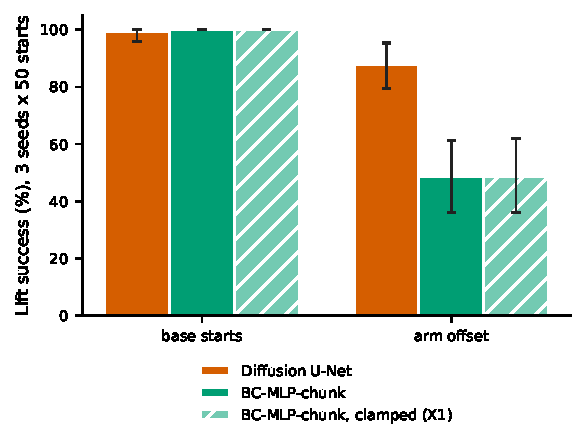
\includegraphics[width=0.6\linewidth]{generated/figures/x1_success.pdf}
\caption{X1, Lift: success on the base and arm-offset robustness sets for diffusion,
BC-MLP-chunk and BC-MLP-chunk with the diffusion sampler's action bound (hatched). The bound
leaves BC-MLP-chunk's success unchanged.}
\label{fig:x1}
\end{figure}

\FloatBarrier
\section{X3: more training seeds on Can, separate replication}
\textbf{Question.} With three seeds, the frozen Can separations H2 (diffusion $-$ BC-MLP) and
H3 (BC-RNN $-$ BC-MLP) held under the preregistered bootstrap but not under a seed-level
interval (KI-053). Do they hold with more seeds, on fresh starts?
\textbf{Design.} The frozen Can configurations were trained with seeds \ax{x3.newseeds}, with
no retuning and with validation-only checkpoint selection. All \ax{x3.nseeds} seeds per family
were then evaluated once on \ax{x3.nstates} new held-out starts, \ax{x3.nevals} evaluations
with \ax{x3.errors} engineering errors.

\textbf{Result} (Table~\ref{tab:x3}, Figure~\ref{fig:contrasts}).
\begin{itemize}
\item H2 diffusion $-$ BC-MLP was \ax{x3.h2bcmlp.b.d}\pp{} [\ax{x3.h2bcmlp.b.lo},
  \ax{x3.h2bcmlp.b.hi}], seed-level [\ax{x3.h2bcmlp.s.lo}, \ax{x3.h2bcmlp.s.hi}]:
  \ax{x3.h2bcmlp.verdict} (\ax{x3.h2bcmlp.relation}).
\item H3 BC-RNN $-$ BC-MLP was \ax{x3.h3.b.d}\pp{}, seed-level [\ax{x3.h3.s.lo},
  \ax{x3.h3.s.hi}]: \ax{x3.h3.verdict}.
\item H2 diffusion $-$ BC-RNN (\ax{x3.h2bcrnn.b.d}\pp) and H2-c diffusion $-$ BC-MLP-chunk
  (\ax{x3.h2c.b.d}\pp) stayed \ax{x3.h2c.verdict}, as in the frozen result.
\end{itemize}
The frozen Level~1 result stands as reported.

\begin{table}[h]
\centering\scriptsize
\caption{X3 (separate replication) beside the frozen Level~1 Can PH values: differences in pp
with bootstrap \ax{level}\pct{} intervals, seed-level \ax{level}\pct{} intervals and verdicts.}
\label{tab:x3}
% Generated by scripts/addendum_assets.py (DECISIONS D-133). Do not edit.
% Every cell is an \ax{} macro of numbers.tex; sources:
%   reports/session13/x1_clamp/results.json ad50368645b96fb87489310243535f97694b1e47a2ff993915b039b2199a5ee7
%   reports/session14/x3/results.json 4299a14930790bfdb2f91d7a3216c9bd7f6db1fa2171469a29bfed3c5c5b71d1
%   reports/session17/x2/results.json 30c01f551333feafba70bfa4c9c6a414eda691f179800022d3871776be2df238
\begin{tabular}{llllp{3.4cm}}
\toprule
Contrast & study & difference, bootstrap & seed-level & verdict \\
\midrule
H2 diffusion $-$ BC-MLP & Level~1 Can PH & \ax{l1.can.h2bcmlp.b.d}\,[\ax{l1.can.h2bcmlp.b.lo}, \ax{l1.can.h2bcmlp.b.hi}] & [\ax{l1.can.h2bcmlp.s.lo}, \ax{l1.can.h2bcmlp.s.hi}] & \ax{l1.can.h2bcmlp.b.sep} \\
 & X3 & \ax{x3.h2bcmlp.b.d}\,[\ax{x3.h2bcmlp.b.lo}, \ax{x3.h2bcmlp.b.hi}] & [\ax{x3.h2bcmlp.s.lo}, \ax{x3.h2bcmlp.s.hi}] & \ax{x3.h2bcmlp.verdict} \\[2pt]
H2 diffusion $-$ BC-RNN & Level~1 Can PH & \ax{l1.can.h2bcrnn.b.d}\,[\ax{l1.can.h2bcrnn.b.lo}, \ax{l1.can.h2bcrnn.b.hi}] & [\ax{l1.can.h2bcrnn.s.lo}, \ax{l1.can.h2bcrnn.s.hi}] & \ax{l1.can.h2bcrnn.b.sep} \\
 & X3 & \ax{x3.h2bcrnn.b.d}\,[\ax{x3.h2bcrnn.b.lo}, \ax{x3.h2bcrnn.b.hi}] & [\ax{x3.h2bcrnn.s.lo}, \ax{x3.h2bcrnn.s.hi}] & \ax{x3.h2bcrnn.verdict} \\[2pt]
H2-c diffusion $-$ BC-MLP-chunk & Level~1 Can PH & \ax{l1.can.h2c.b.d}\,[\ax{l1.can.h2c.b.lo}, \ax{l1.can.h2c.b.hi}] & [\ax{l1.can.h2c.s.lo}, \ax{l1.can.h2c.s.hi}] & \ax{l1.can.h2c.b.sep} \\
 & X3 & \ax{x3.h2c.b.d}\,[\ax{x3.h2c.b.lo}, \ax{x3.h2c.b.hi}] & [\ax{x3.h2c.s.lo}, \ax{x3.h2c.s.hi}] & \ax{x3.h2c.verdict} \\[2pt]
H3 BC-RNN $-$ BC-MLP & Level~1 Can PH & \ax{l1.can.h3.b.d}\,[\ax{l1.can.h3.b.lo}, \ax{l1.can.h3.b.hi}] & [\ax{l1.can.h3.s.lo}, \ax{l1.can.h3.s.hi}] & \ax{l1.can.h3.b.sep} \\
 & X3 & \ax{x3.h3.b.d}\,[\ax{x3.h3.b.lo}, \ax{x3.h3.b.hi}] & [\ax{x3.h3.s.lo}, \ax{x3.h3.s.hi}] & \ax{x3.h3.verdict} \\[2pt]
\bottomrule
\end{tabular}

\end{table}

\FloatBarrier
\section{X2 (Can MH): mixed-quality demonstrations}
\textbf{Question.} The frozen tasks sit near the ceiling, and the proficient-human data are
nearly unimodal. Does the generative head help when the demonstrations come from several
operators of different quality, on the task, simulator and controller already validated for
Can?
\textbf{Design.} The robomimic Can MH demonstrations were split by robomimic's
operator-stratified masks, so every operator appears in training and validation. Each family
was tuned with the frozen Level~1 budget and selected on validation starts only. The
\ax{x2.nevals} chosen checkpoints (\ax{x2.nseeds} seeds per family) were then evaluated once on
\ax{x2.nstates} new held-out starts, after a freeze committed alone. There were
\ax{x2.errors} engineering errors and no rerun.

\textbf{Result} (Tables~\ref{tab:x2}, \ref{tab:fam} and \ref{tab:cens},
Figure~\ref{fig:contrasts}).
\begin{itemize}
\item Diffusion reached \ax{x2.fam.diff.succ}\pct, BC-MLP-chunk \ax{x2.fam.chunk.succ}\pct,
  BC-RNN \ax{x2.fam.bcrnn.succ}\pct{} and BC-MLP \ax{x2.fam.bcmlp.succ}\pct.
\item H2 diffusion $-$ BC-MLP (\ax{x2.h2bcmlp.b.d}\pp) and H3 BC-RNN $-$ BC-MLP
  (\ax{x2.h3.b.d}\pp) were \ax{x2.h3.verdict}, the same direction as on Can PH.
\item H2 diffusion $-$ BC-RNN was \ax{x2.h2bcrnn.b.d}\pp{} [\ax{x2.h2bcrnn.b.lo},
  \ax{x2.h2bcrnn.b.hi}], seed-level [\ax{x2.h2bcrnn.s.lo}, \ax{x2.h2bcrnn.s.hi}]:
  \ax{x2.h2bcrnn.verdict}. This is a \ax{x2.h2bcrnn.relation} relative to Can PH.
\item H2-c diffusion $-$ BC-MLP-chunk was \ax{x2.h2c.b.d}\pp{} [\ax{x2.h2c.b.lo},
  \ax{x2.h2c.b.hi}]: \ax{x2.h2c.verdict} (\ax{x2.h2c.relation}).
\item Episodes in which the gripper never closed: BC-MLP \ax{x2.tax.bcmlp.gripper-never-closed},
  diffusion \ax{x2.tax.diff.gripper-never-closed}.
\end{itemize}

\textbf{Reading.} On these mixed-quality data, the recurrent policy falls well behind both
chunked policies, and the one-step MLP further still. The two policies that predict
\emph{chunks} of future actions, one by denoising and one deterministically, are not
separated. These are within-operator results on the X2 held-out starts. They do not measure
transfer to a new operator, and they do not change the frozen Can PH numbers or their
fragility (KI-053).

\begin{table}[h]
\centering\scriptsize
\caption{X2 (Can MH) beside the frozen Level~1 Can PH values (never pooled; different data,
starts and horizon): differences in pp with bootstrap and seed-level \ax{level}\pct{} intervals.}
\label{tab:x2}
% Generated by scripts/addendum_assets.py (DECISIONS D-133). Do not edit.
% Every cell is an \ax{} macro of numbers.tex; sources:
%   reports/session13/x1_clamp/results.json ad50368645b96fb87489310243535f97694b1e47a2ff993915b039b2199a5ee7
%   reports/session14/x3/results.json 4299a14930790bfdb2f91d7a3216c9bd7f6db1fa2171469a29bfed3c5c5b71d1
%   reports/session17/x2/results.json 30c01f551333feafba70bfa4c9c6a414eda691f179800022d3871776be2df238
\begin{tabular}{llllp{3.4cm}}
\toprule
Contrast & study & difference, bootstrap & seed-level & verdict \\
\midrule
H2 diffusion $-$ BC-MLP & Level~1 Can PH & \ax{l1.x2side.h2bcmlp.b.d}\,[\ax{l1.x2side.h2bcmlp.b.lo}, \ax{l1.x2side.h2bcmlp.b.hi}] & [\ax{l1.x2side.h2bcmlp.s.lo}, \ax{l1.x2side.h2bcmlp.s.hi}] & \ax{l1.x2side.h2bcmlp.b.sep} \\
 & X2 (Can MH) & \ax{x2.h2bcmlp.b.d}\,[\ax{x2.h2bcmlp.b.lo}, \ax{x2.h2bcmlp.b.hi}] & [\ax{x2.h2bcmlp.s.lo}, \ax{x2.h2bcmlp.s.hi}] & \ax{x2.h2bcmlp.verdict}; \ax{x2.h2bcmlp.relation} \\[2pt]
H2 diffusion $-$ BC-RNN & Level~1 Can PH & \ax{l1.x2side.h2bcrnn.b.d}\,[\ax{l1.x2side.h2bcrnn.b.lo}, \ax{l1.x2side.h2bcrnn.b.hi}] & [\ax{l1.x2side.h2bcrnn.s.lo}, \ax{l1.x2side.h2bcrnn.s.hi}] & \ax{l1.x2side.h2bcrnn.b.sep} \\
 & X2 (Can MH) & \ax{x2.h2bcrnn.b.d}\,[\ax{x2.h2bcrnn.b.lo}, \ax{x2.h2bcrnn.b.hi}] & [\ax{x2.h2bcrnn.s.lo}, \ax{x2.h2bcrnn.s.hi}] & \ax{x2.h2bcrnn.verdict}; \ax{x2.h2bcrnn.relation} \\[2pt]
H2-c diffusion $-$ BC-MLP-chunk & Level~1 Can PH & \ax{l1.x2side.h2c.b.d}\,[\ax{l1.x2side.h2c.b.lo}, \ax{l1.x2side.h2c.b.hi}] & [\ax{l1.x2side.h2c.s.lo}, \ax{l1.x2side.h2c.s.hi}] & \ax{l1.x2side.h2c.b.sep} \\
 & X2 (Can MH) & \ax{x2.h2c.b.d}\,[\ax{x2.h2c.b.lo}, \ax{x2.h2c.b.hi}] & [\ax{x2.h2c.s.lo}, \ax{x2.h2c.s.hi}] & \ax{x2.h2c.verdict}; \ax{x2.h2c.relation} \\[2pt]
H3 BC-RNN $-$ BC-MLP & Level~1 Can PH & \ax{l1.x2side.h3.b.d}\,[\ax{l1.x2side.h3.b.lo}, \ax{l1.x2side.h3.b.hi}] & [\ax{l1.x2side.h3.s.lo}, \ax{l1.x2side.h3.s.hi}] & \ax{l1.x2side.h3.b.sep} \\
 & X2 (Can MH) & \ax{x2.h3.b.d}\,[\ax{x2.h3.b.lo}, \ax{x2.h3.b.hi}] & [\ax{x2.h3.s.lo}, \ax{x2.h3.s.hi}] & \ax{x2.h3.verdict}; \ax{x2.h3.relation} \\[2pt]
\bottomrule
\end{tabular}

\end{table}

\begin{table}[h]
\centering\scriptsize
\caption{Family success (\%) with bootstrap \ax{level}\pct{} intervals, in separate columns: the frozen
Level~1 Can PH result, X3 and X2 (Can MH). The X2 column is on a different dataset, start
suite and horizon.}
\label{tab:fam}
% Generated by scripts/addendum_assets.py (DECISIONS D-133). Do not edit.
% Every cell is an \ax{} macro of numbers.tex; sources:
%   reports/session13/x1_clamp/results.json ad50368645b96fb87489310243535f97694b1e47a2ff993915b039b2199a5ee7
%   reports/session14/x3/results.json 4299a14930790bfdb2f91d7a3216c9bd7f6db1fa2171469a29bfed3c5c5b71d1
%   reports/session17/x2/results.json 30c01f551333feafba70bfa4c9c6a414eda691f179800022d3871776be2df238
\begin{tabular}{lllll}
\toprule
Family & Level~1 Can PH (frozen) & X3 & X2 (Can MH) & X2 per seed \\
 & \ax{l1.can.fam.diff.nseeds} seeds $\times$ \ax{l1.can.fam.diff.nstates}, \ax{l1.horizon} steps & \ax{x3.nseeds} seeds $\times$ \ax{x3.nstates}, \ax{l1.horizon} steps & \ax{x2.nseeds} seeds $\times$ \ax{x2.nstates}, \ax{x2.horizon} steps & \% \\
\midrule
Diffusion U-Net & \ax{l1.can.fam.diff.succ} [\ax{l1.can.fam.diff.lo}, \ax{l1.can.fam.diff.hi}] & \ax{x3.fam.diff.succ} [\ax{x3.fam.diff.lo}, \ax{x3.fam.diff.hi}] & \ax{x2.fam.diff.succ} [\ax{x2.fam.diff.lo}, \ax{x2.fam.diff.hi}] & \ax{x2.fam.diff.perseed} \\
BC-MLP-chunk & \ax{l1.can.fam.chunk.succ} [\ax{l1.can.fam.chunk.lo}, \ax{l1.can.fam.chunk.hi}] & \ax{x3.fam.chunk.succ} [\ax{x3.fam.chunk.lo}, \ax{x3.fam.chunk.hi}] & \ax{x2.fam.chunk.succ} [\ax{x2.fam.chunk.lo}, \ax{x2.fam.chunk.hi}] & \ax{x2.fam.chunk.perseed} \\
BC-RNN & \ax{l1.can.fam.bcrnn.succ} [\ax{l1.can.fam.bcrnn.lo}, \ax{l1.can.fam.bcrnn.hi}] & \ax{x3.fam.bcrnn.succ} [\ax{x3.fam.bcrnn.lo}, \ax{x3.fam.bcrnn.hi}] & \ax{x2.fam.bcrnn.succ} [\ax{x2.fam.bcrnn.lo}, \ax{x2.fam.bcrnn.hi}] & \ax{x2.fam.bcrnn.perseed} \\
BC-MLP & \ax{l1.can.fam.bcmlp.succ} [\ax{l1.can.fam.bcmlp.lo}, \ax{l1.can.fam.bcmlp.hi}] & \ax{x3.fam.bcmlp.succ} [\ax{x3.fam.bcmlp.lo}, \ax{x3.fam.bcmlp.hi}] & \ax{x2.fam.bcmlp.succ} [\ax{x2.fam.bcmlp.lo}, \ax{x2.fam.bcmlp.hi}] & \ax{x2.fam.bcmlp.perseed} \\
\bottomrule
\end{tabular}

\end{table}

\begin{table}[h]
\centering\small
\caption{X2 (Can MH), declared secondary without readings: censored episode length (first
success step, else the horizon).}
\label{tab:cens}
% Generated by scripts/addendum_assets.py (DECISIONS D-133). Do not edit.
% Every cell is an \ax{} macro of numbers.tex; sources:
%   reports/session13/x1_clamp/results.json ad50368645b96fb87489310243535f97694b1e47a2ff993915b039b2199a5ee7
%   reports/session14/x3/results.json 4299a14930790bfdb2f91d7a3216c9bd7f6db1fa2171469a29bfed3c5c5b71d1
%   reports/session17/x2/results.json 30c01f551333feafba70bfa4c9c6a414eda691f179800022d3871776be2df238
\begin{tabular}{lll}
\toprule
Contrast & difference (steps, \ax{level}\,\%) & verdict \\
\midrule
H2 diffusion $-$ BC-MLP & \ax{x2.cens.h2bcmlp.d}\,[\ax{x2.cens.h2bcmlp.lo}, \ax{x2.cens.h2bcmlp.hi}] & \ax{x2.cens.h2bcmlp.sep} \\
H2 diffusion $-$ BC-RNN & \ax{x2.cens.h2bcrnn.d}\,[\ax{x2.cens.h2bcrnn.lo}, \ax{x2.cens.h2bcrnn.hi}] & \ax{x2.cens.h2bcrnn.sep} \\
H2-c diffusion $-$ BC-MLP-chunk & \ax{x2.cens.h2c.d}\,[\ax{x2.cens.h2c.lo}, \ax{x2.cens.h2c.hi}] & \ax{x2.cens.h2c.sep} \\
H3 BC-RNN $-$ BC-MLP & \ax{x2.cens.h3.d}\,[\ax{x2.cens.h3.lo}, \ax{x2.cens.h3.hi}] & \ax{x2.cens.h3.sep} \\
\bottomrule
\end{tabular}

\end{table}

\begin{figure}[h]
\centering
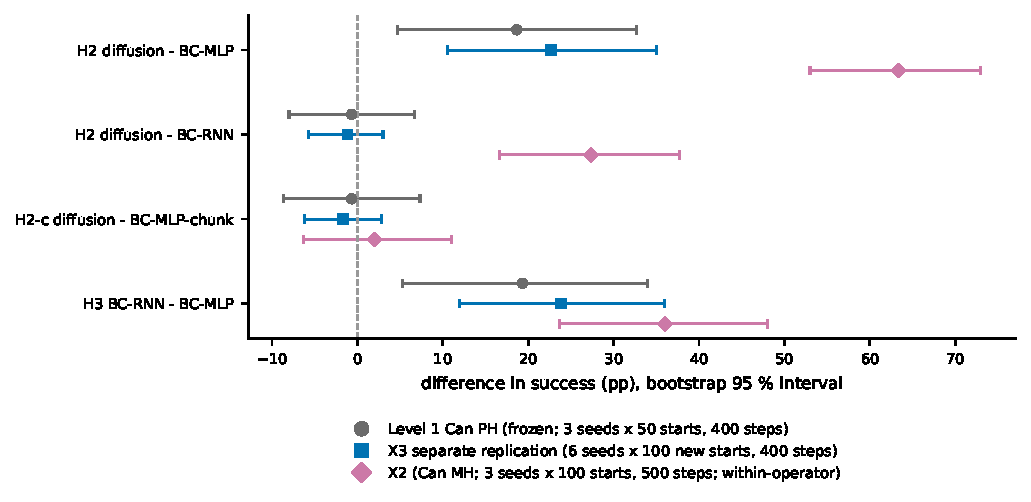
\includegraphics[width=\linewidth]{generated/figures/contrasts.pdf}
\caption{The four declared Can contrasts: frozen Level~1 Can PH (circles), X3 (squares) and
X2 (Can MH, diamonds), each with its bootstrap \ax{level}\pct{} interval. The three are shown beside
each other and never pooled.}
\label{fig:contrasts}
\end{figure}

\FloatBarrier
\section{What changes, and what does not}
\begin{itemize}
\item The v1.0.0 results, freezes and report are unchanged.
\item H2-c was not separated in the frozen Can PH result, in X3 and in X2 (and on Lift in the
  v1.0.0 report). Across these data, the diffusion head shows no measurable gain over a
  deterministic head with the same observation history and action chunks.
\item The BC side of the action-bound confound (KI-052) is resolved: BC's missing bound does
  not explain the robustness gaps. The diffusion side is open.
\item The fragile Can PH separations hold in a larger replication (X3).
\item With mixed-quality demonstrations (X2), chunked policies separate from the recurrent and
  one-step baselines by wide margins.
\end{itemize}

\section{Limitations}
Simulation only, with exact object state as input. The studies use small diffusion models,
the frozen tuning budgets, a few seeds and a single canonical platform. X1 used validation-regime
starts and one action bound. X3 replicated Can only. X2 is within-operator, uses a
\ax{x2.horizon}-step horizon and one task. This addendum, like the v1.0.0 report, is a local
build and has not been peer reviewed.

\section*{Reproduction}
\file{make addendum-check} regenerates every table, figure and macro from the pinned files and
compares them byte for byte; \file{make addendum} builds this PDF with the v1.0.0 toolchain.
The study records are \file{docs/extensions/}, \file{docs/DECISIONS.md} (D-105 to D-134) and
\file{docs/EXPERIMENT_LEDGER.md}.

\bibliographystyle{plainnat}
\bibliography{../references}
\end{document}
